
\documentclass[calculator,steamtables,datasheet,solutions]{exam_newMarcus2}
%\documentclass[calculator,steamtables,allquestions,datasheet,resit]{exam_newMarcus2}

% The full list of class options are
% calculator : Allows approved calculator use.
% datasheet : Adds a note that data sheet are attached to the exam.
% handbook : Allows the use of the engineering handbook.
% resit : Adds the resit markings to the paper.
% sample : Adds conspicuous SAMPLE markings to the paper
% solutions : Uses the contents of \solution commands (and \solmarks) to generate a solution file

\usepackage{pdfpages}  
\usepackage{lscape,comment}
 
\coursecode{EX3029}%%
\coursetitle{Chemical Thermodynamics}

\examtime{09.00--12.00}%
\examdate{03}{06}{2016}% 
\examformat{Candidates must attempt \textit{all} questions.}

\newcommand{\frc}{\displaystyle\frac}
\newcommand{\br}[1]{\!\left( #1 \right)}
\newcommand{\abs}[1]{\left| #1 \right|}
\newcommand{\fracd}[2]{\frac{\mathrm{d} #1}{\mathrm{d} #2}}
\newcommand{\fracp}[2]{\frac{\partial #1}{\partial #2}}
\renewcommand{\d}[1]{\mathrm{d} #1 } 
\newcommand{\Ma}{\mathrm{M\!a}} 



\begin{document}

%%%
%%% Question 01
%%%
\begin{question}
%
\begin{enumerate}[(a)]

% (Shapiro 2.34) 
\item Air contained in a piston-cylinder system undergoes three consecutive processes,
\begin{itemize} 
\item Process 1--2: Isobaric cooling with P$_{1}$=69 kPa and V$_{1}$=0.11 m$^{3}$;
\item Process 2--3: Isochoric heating with P$_{3}$=345 kPa;
\item Process 3--1: Polytropic expansion, with $PV=$ {\it constant}. %Expansion to the initial state, during which the pressure-volume relationship is $PV=$ {\it constant}.
\end{itemize}  
\begin{enumerate}[(i)]
\item Calculate V$_{2}$ $\left(\text{in m}^{3}\right)$.~\marks{3} 
\solution{
For Process 2--3: V$_{2}$=V$_{3}$. However the expansion 3--1 follows $PV=$ constant,
\begin{displaymath}
P_{1}V_{1}=P_{3}V_{3} \Longrightarrow V_{3} = \frc{P_{1}V_{1}}{P_{3}} = {\bf 0.022\;\text{m}^{3} = V_{2}}
\end{displaymath}~\solmarks{3/3}
}
\item Calculate the work (in $kJ$) for each process.~\marks{6}
\solution{\noindent
Process 1--2: 
\begin{displaymath}
{\bf W_{1-2}} = \int\limits_{V_{1}}^{V_{2}} P dV = P\left(V_{2}-V_{1}\right) = -6072 J \Rightarrow {\bf -6.072 kJ}
\end{displaymath}~\solmarks{2/6}
\noindent
Process 2--3: V$_{2}$=V$_{3}$ $\Longrightarrow$ {\bf W$_{2-3}$ = 0}~\solmarks{2/6} \\
\noindent
Process 3--1: $PV = C$
\begin{displaymath} 
{\bf W_{31}} = \int\limits_{V_{3}}^{V_{1}}P dV = \int\limits_{V_{3}}^{V_{1}}\frc{C}{V} dV = P_{1}V_{1}\ln\frc{V_{1}}{V_{3}} = 12220 J \Rightarrow {\bf 12.22 kJ} 
\end{displaymath}~\solmarks{2/6}
}
\item Sketch the $PV$ diagram for these processes.~\marks{4}
\solution{\solmarks{4/4}
\begin{center}
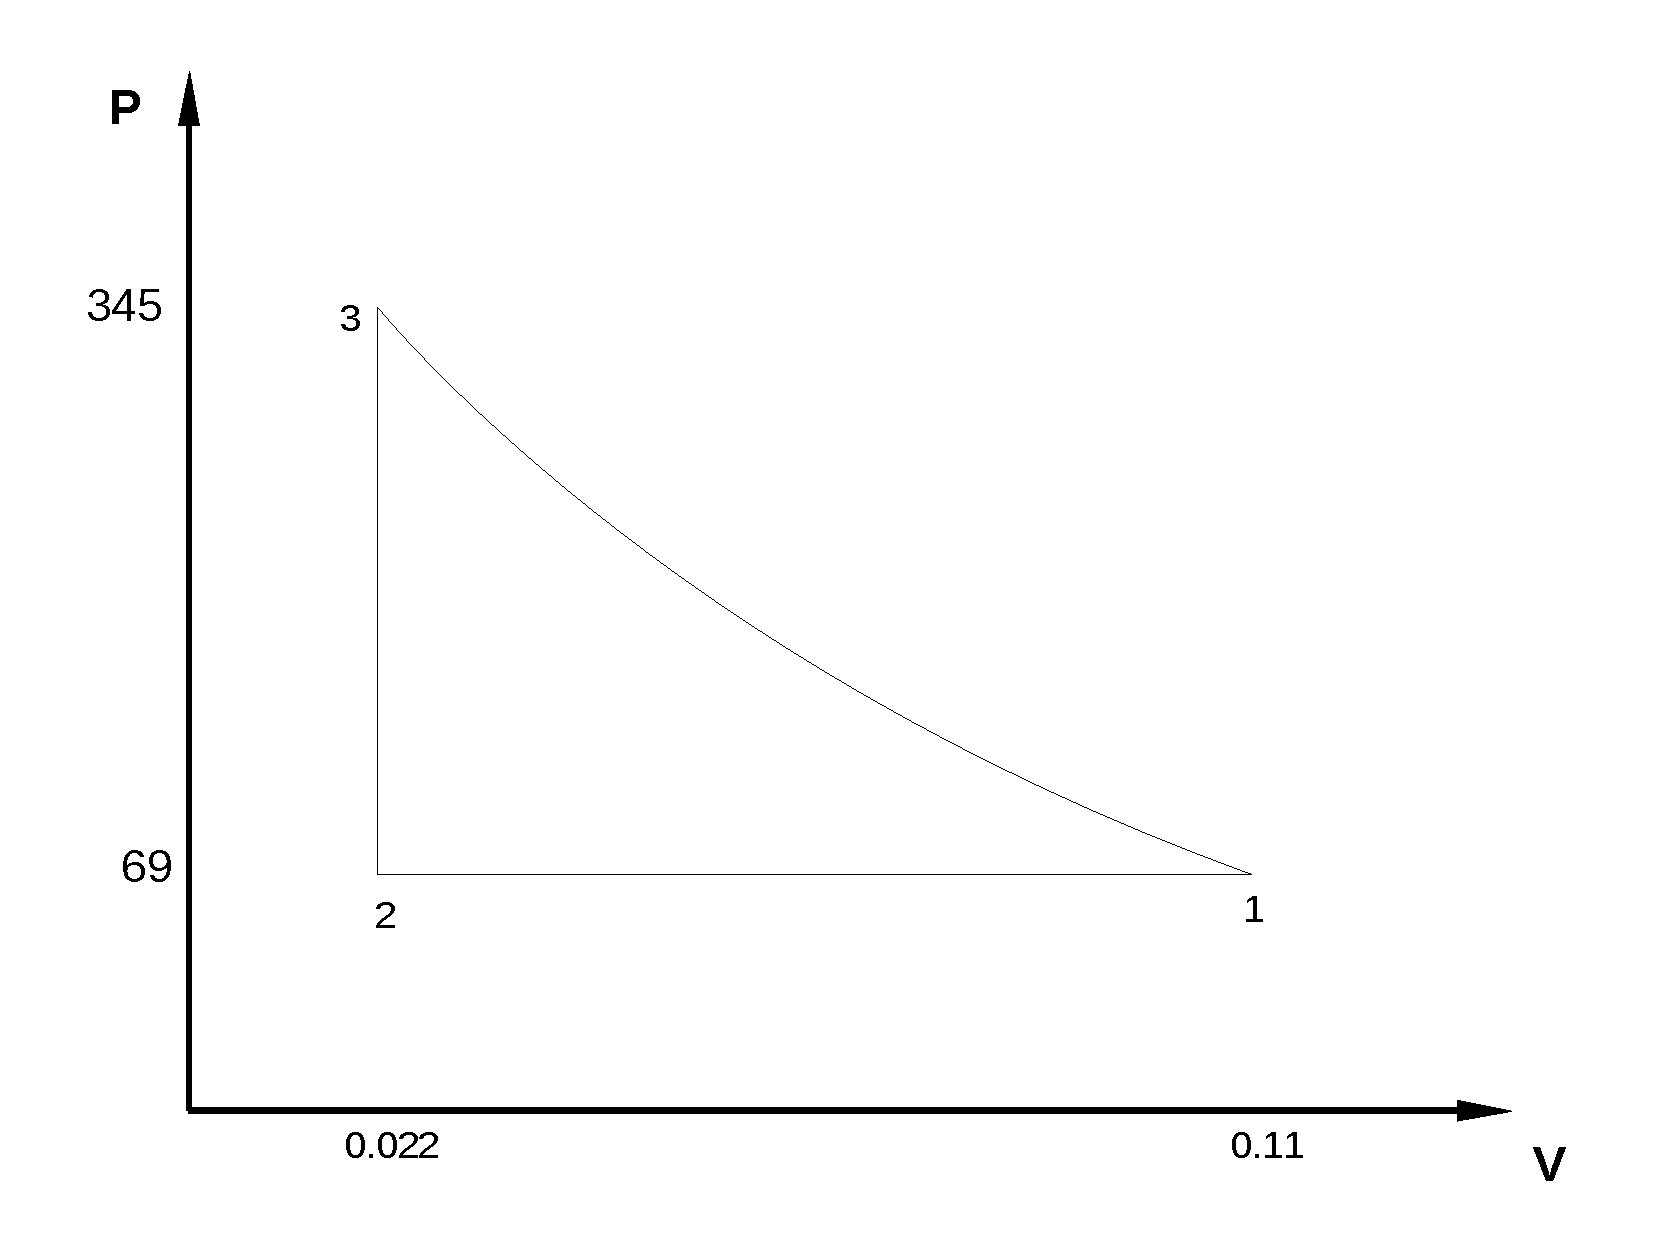
\includegraphics[width=10.cm,height=8.cm,clip]{./Pics/Exam_PV_Diagram}
\end{center}
}
\end{enumerate}

%
\item Calculate the fugacity of steam at 300$^{\circ}$C and 80 bar. For your calculations, you should use $h=$ 2785 kJ/kg, $s=$ 5.791 kJ/(kg.K) for steam at 300$^{\circ}$C and 80 bar. Specific enthalpy and entropy of ideal gas at 300$^{\circ}$C and 0.1 bar are $h^{\text{IG}}=$ 3077 kJ/kg and $s^{\text{IG}}=$ 9.281 kJ/(kg.K), respectively. Given,
\begin{displaymath}
 d\mu = dG = RTd\left(\ln{f}\right).
\end{displaymath} 
Also, molar mass of water is 18 g/mol.~\marks{7}

%=======================
\solution{ We can integrate this equation from low pressure so that fugacity is similar to pressure and the system can be considered an ideal gas,\solmarks{2/7}
\begin{displaymath}
\int\limits_{G^{\text{IG}}}^{G}dG = RT\int\limits_{P}^{f}d\left(\ln{f}\right) \Longrightarrow f = P\exp{\left(\frc{G-G^{\text{IG}}}{RT}\right)}
\end{displaymath}
The specific gibbs free energy of ideal gas (at low pressure, e.g., 0.1 bar)~\solmarks{1/7}
\begin{displaymath}
g^{\text{IG}} = h^{\text{IG}}-Ts^{\text{IG}} = -2242.41 kJ/kg \Longrightarrow G^{\text{IG}} = -40.36 kJ/mol
\end{displaymath}
Now at 300$^{\circ}$C and 80 bar,~\solmarks{1/7}
\begin{displaymath}
g = h - Ts = -534.11 kJ/kg \Longrightarrow G = -9.61 kJ/mol
\end{displaymath}
Now calculating the fugacity,~\solmarks{3/7}
\begin{displaymath}
f = P\exp{\left(\frc{G-G^{\text{IG}}}{RT}\right)} = 63.47 bar
\end{displaymath}
}
%=======================
%
\end{enumerate}
%
\end{question}
\clearpage

%%%
%%% Question 02
%%%
\begin{question}
%
\begin{enumerate}[(a)]
%
\item Develop expressions for the volume expansivity, $\beta=\frc{1}{V}\left(\frc{\partial V}{\partial T}\right)_{P}$, and isothermal compressibility, $\kappa=-\frc{1}{V}\left(\frc{\partial V}{\partial P}\right)_{T}$, for the following equations of state,
\begin{enumerate}[(i)]
\item ideal gas~\marks{4}
\solution{Ideal gas: $V=\frc{RT}{P}$,
\begin{displaymath}
\left(\frc{\partial V}{\partial T}\right)_{P} = \frc{R}{P} \;\;\; \left(\frc{\partial V}{\partial P}\right)_{T} = -\frc{RT}{P^{2}} 
\end{displaymath}~\solmarks{2/4}
Now deriving $\beta$ and $\kappa$,
\begin{displaymath}
{\bf \beta} = \frc{1}{V}\frc{R}{P} {\bf = \frc{1}{T}}\;\;\text{ and}\;\;\kappa = -\frc{1}{V}\left(-\frc{RT}{P^{2}}\right){\bf = \frc{1}{P}}
\end{displaymath}~\solmarks{2/4}
}
\item $V=\frc{RT}{P}+b$~\marks{4}
\solution{
The derivatives are,
\begin{displaymath}
\left(\frc{\partial V}{\partial T}\right)_{P} = \frc{R}{P} \;\;\; \left(\frc{\partial V}{\partial P}\right)_{T} = -\frc{RT}{P^{2}} 
\end{displaymath}~\solmarks{2/4}
Now deriving $\beta$ and $\kappa$,
\begin{displaymath} 
{\bf \beta} = \frc{1}{V}\frc{R}{P} =\frc{R}{V}\frc{V-b}{RT}= {\bf = \frc{1}{T}\frc{V-b}{V}} \;\;\text{ and }\;\; {\bf \kappa} = -\frc{1}{V}\left(-\frc{RT}{P^{2}}\right){\bf = \frc{1}{P}\left[\frc{V-b}{V}\right]}
\end{displaymath}~\solmarks{2/4}
}
\end{enumerate}

\item Calculate the compressibility factor ($Z$) and molar volume of sulphur dioxide $\left(SO_{2}\right)$ vapour at 300 K and 4 bar using the Redlich-Kwong equation of state. Properties of SO$_{2}$ are: T$_{c}$ = 430 K, P$_{c}$ = 78.7 bar and $\omega$ = 0.251 (accentric factor). In your iterative calculations, use $Z_{0}=1$ as initial guess of $Z$, and stop at the second iteration $\left(Z_{2}\right)$.~\marks{12}
\solution{ The generic form of $Z$ is,
\begin{displaymath}
Z = 1+ \beta - q\beta\frc{Z - \beta}{\left(Z+\epsilon\beta\right)\left(Z+\sigma\beta\right)}\;\;\text{ with} \;\; \beta = \Omega \frc{P_{r}}{T_{r}}\;\;\text{ and}\;\; q=\frc{\Psi\alpha}{\Omega T_{r}}
\end{displaymath}
For SRK with {\bf T$_{r}$=0.8380}, {\bf P$_{r}$=0.3754}, {\bf $\beta$=3.88$\times$10$^{-2}$} and {\bf $q$=6.7274}~\solmarks{2/12},
\begin{displaymath}
{\bf Z = 1 + \beta - q\beta\frc{Z-\beta}{Z^{2}+\beta Z}}
\end{displaymath}~\solmarks{2/12}
The equation is non-linear and to find the root we can apply Newton-Raphson method 
\begin{displaymath}
Z_{i} = Z_{i-1} - \frc{\mathcal{F}\left(Z_{i-1}\right)}{d\mathcal{F}/dZ \left(Z_{i-1}\right)}
\end{displaymath}
with,
\begin{eqnarray}
&& \mathcal{F}\left(Z\right) = Z - \left[ 1 + \beta - q\beta\frc{Z-\beta}{Z^{2}+\beta Z}\right] \nonumber \\
&& \frc{d\mathcal{F}}{dZ}\left(Z\right) = 1 + q\beta \frc{\beta^{2}+2\beta Z- Z^{2}}{\left(Z^{2}+\beta Z\right)^{2}} \nonumber
%\frc{q\beta\left(Z^{2}\beta +Z\right)-q\beta Z\left(2Z + \beta\right)}{\left(Z^{2}+\beta Z\right)^{2}} + \frc{q\beta^{2}\left(2Z+\beta\right)}{\left(Z^{2}+\beta Z\right)^{2}} \nonumber
\end{eqnarray} 
as initial guess, we can use the generic real gas EOS, $PV=Z_{0}RT \Longrightarrow$ {\bf $Z_{0}=0.7217$}~\solmarks{2/12}. Thus 
\begin{center}
{\bf $Z_{1}$ = 0.7184}~\solmarks{3/12} \\
{\bf $Z_{2}$ = 0.7160}~\solmarks{3/12} \\
$\cdots \cdots \cdots $ \\
\textcolor{red} {or (using calculator) }{\bf $Z_{22}$ = 0.7088}~\solmarks{\textcolor{red}{8/12}} \\

\end{center}
} 
%
\end{enumerate}
%
\end{question}

\clearpage

%%%
%%% Question 03
%%%
\begin{question}
%
\begin{enumerate}[(a)]
%%%
%%% Johannes T0902
%%%
\item\label{T0902} Assuming that all species and their mixtures are ideal gases, derive an equation for the Gibbs energy as a function of the reaction coordinate for the reaction below at 1000K.
\begin{displaymath}
H_{2} + CO_{2} \Longleftrightarrow H_{2}O + CO
\end{displaymath}
Calculate the reaction coordinate, $\epsilon$, in the equilibrium.
Given $\Delta G_{f}^{\circ}$ $\left(\text{J.gmol}^{-1}\right)$ at 1000K: (a) H$_{2}$O: -192420, (b) CO: -200240 and (c) CO$_{2}$: -395790.~\marks{13}

%==========================
\solution{ The Gibbs energy can be expressed as~\solmarks{1/13}
\begin{eqnarray}
G &=& \sum y_{i}G_{i} + RT\sum y_{i}\ln{y_{i}} \nonumber \\
G &=& \sum y_{i}\Delta G^{o}_{f,i} + RT\sum y_{i}\ln{y_{i}} \nonumber 
\end{eqnarray}
We can differentiate the total Gibbs energy as,
\begin{displaymath}
dG^{t} = d\left(n G\right) = n\frc{dG}{d\epsilon} + G\frc{d n}{d\epsilon} 
\end{displaymath} 
Assuming the system is closed and in equilibrium: $dn = 0$ and $\frc{dG}{d\epsilon}=0$. For 1 mole of H$_{2}$ and CO$_{2}$, the mole fraction of the gaseous species are~\solmarks{1/13}
\begin{displaymath}
y_{\text{H}_{2}}=\frc{1-\epsilon}{2} =y_{\text{CO}_{2}}\;\;\text{ and }\;\; y_{\text{H}_{2}\text{O}}=\frc{\epsilon}{2} =y_{\text{CO}}\
\end{displaymath}
Thus,~\solmarks{5/13}
\begin{eqnarray}
 G &=& \left(y_{H_{2}}\Delta G^{o}_{f,H_{2}} + y_{CO_{2}}\Delta G^{o}_{f,CO_{2}} + y_{H_{2}O}\Delta G^{o}_{f,H_{2}O} + y_{CO}\Delta G^{o}_{f,CO}\right) + \nonumber \\
    && RT\left(y_{H_{2}}\ln{y_{H_{2}}} + y_{CO_{2}}\ln{y_{CO_{2}}} + y_{H_{2}O}\ln{y_{H_{2}O}} + y_{CO}\ln{y_{CO}}\right) \nonumber \\
   &=&\left[\frc{1-\epsilon}{2}\Delta G^{o}_{f,CO_{2}} + \frc{\epsilon}{2}\left(\Delta G^{o}_{f,H_{2}O}+\Delta G^{o}_{f,CO}\right)\right] + RT\left[\left(1-\epsilon\right)\ln{\frc{1-\epsilon}{2}} + \epsilon\ln{\frc{\epsilon}{2}}\right]\nonumber
\end{eqnarray}
for $\Delta G^{o}_{f,H_{2}} = 0$. In the equilibrium $\frc{dG}{d\epsilon}=0$~\solmarks{1/13}, therefore~\solmarks{5/13}
\begin{displaymath}
\frc{dG}{d\epsilon} = B-A + RT\left[\ln{\frc{\epsilon}{2}} - \ln{\frc{1-\epsilon}{2}}\right] = 0 \Longrightarrow \epsilon = 0.4531 
\end{displaymath}
with $A=\frc{-395790}{2}$ and $B=\frc{-192420-200240}{2}$.
}
%==========================
%

%%%
%%% Problem 8.3 (Power Lectures Notes)
%%%
\item Saturated ammonia $\left(\text{NH}_{3}\right)$ vapour at $P_{1} = 200$ kPa is compressed by a piston to $P_{2} = 1.6$ MPa in a reversible adiabatic process. Calculate the work done per unit mass.~\marks{7}

%=========================
\solution{At 200 kPa (2 bar), from the saturated tables:~\solmarks{2/7}
\begin{center}
\begin{tabular}{c c } 
 $v_{1}=0.5946\;m^{3}/kg$ &$T_{1}=-18.86^{\circ}C$ \\
 $s_{1}=5.5969\;kJ/(kg.K)$ & $u_{1}=1300.39\;kJ/kg$\\
\end{tabular}
\end{center}
Reversible and adiabatic compresion implied in isentropic process, therefore $s_{2}=s_{1}$. At  $P_{2}=1.6\text{ MPa}=16\text{ bar}$, the specific entropy of saturated ammonia vapour is 4.8542 kJ/(kg.K), which is smaller than $s_{1}$, indicating that the fluid is at superheated state. With $P_{2}$ and $s_{2}$, in the superheated fluid table we can obtain (through linear interpolation),~\solmarks{2/7}
\begin{center}
\begin{tabular}{c c } 
 $v_{2}=0.1180\;m^{3}/kg$ &$T_{2}=135.16^{\circ}C$ \\
 $s_{2}=5.5969\;kJ/(kg.K)$ & $u_{2}=1546.50\;kJ/kg$\\
\end{tabular}
\end{center}
From the First Law,~\solmarks{3/7}
\begin{eqnarray}
   && \Delta u = q + w \text{ with } q=0 \text{ because the process is adiabatic} \nonumber \\
   && w = u_{2}-u_{1} = 246.11 \text{kJ/kg (positive because work is given to the system).}\nonumber
\end{eqnarray}


}
%=========================


\end{enumerate}
%
\end{question}

\clearpage

%%%
%%% Question 04
%%%
\begin{question}

 Estimate the bubble and dew point temperatures of a 25 mol-$\%$ n-pentane $\left(nC_{5}\right)$, 45 mol-$\%$ n-hexane $\left(nC_{6}\right)$ and 30 mol-$\%$ n-heptane $\left(nC_{7}\right)$ mixture at 1.013 bar. Also calculate the compositions at dew and bubble points. ~\marks{20}
\solution{ iouh}

For This problem, use 
\begin{displaymath}
   \ln P_{i}^{\text{sat}} = A_{i} - \frc{B_{i}}{RT}
\end{displaymath} 
with [P] = bar and [T] = K, and
    \begin{center}
       \begin{tabular}{l l l} 
          $A_{nC_{5}}=10.422$ & $A_{nC_{6}}=10.456$ & $A_{nC_{7}}=11.431$ \\
          $B_{nC_{5}}=26799$  & $B_{nC_{6}}=29676$  & $B_{nC_{7}}=35200$  
       \end{tabular}
    \end{center}
If you are using an iterative method to solve this problem, do stop at the 5$^{th}$ iteration.

%=======================
\solution{For the bubble point, we need to solve~\solmarks{2/20}
\begin{displaymath}
\sum\limits_{i=1}^{3} y_{i} = 1 = \frc{x_{C5}P_{C5}^{sat}}{P} + \frc{x_{C6}P_{C6}^{sat}}{P} + \frc{x_{C7}P_{C7}^{sat}}{P}  
\end{displaymath}
for $T$, with 
\begin{displaymath}
   \ln P_{i}^{\text{sat}} = A_{i} - \frc{B_{i}}{RT}.
\end{displaymath} 
Leading to $T=334.94$ K (at the 5$^{th}$ iteration)~\solmarks{5/20} with composition $y = \left[0.5483\; 0.0883\; 0.3634\right]$ for n-pentane, n-hexane and n-heptane, respectively.~\solmarks{3/20}.

For the dew point, we need to  solve~\solmarks{2/20}
\begin{displaymath}
\sum\limits_{i=1}^{3} x_{i} = 1 = \frc{y_{C5}P}{P_{C5}^{sat}} + \frc{y_{C6}P}{P_{C6}^{sat}} + \frc{y_{C7}P}{P_{C7}^{sat}}  
\end{displaymath}
for $T$, leading to $T=350.58$ K (at the 5$^{th}$ iteration)~\solmarks{5/20} with composition $x = \left[0.0742\; 0.3463\; 0.5795\right]$.~\solmarks{3/20}

}
%=======================
%
\end{question}

\clearpage

%%%
%%% Question 05
%%%
\begin{question}
%
\begin{enumerate}[(a)]

%%% Johannes T0602
%%%
\item\label{T0602} What is the change in entropy when 700 litres of CO$_{2}$ and 300 litres of N$_{2}$, each at 1 bar and 25$^{\circ}$C, blend to form a gas mixture at the same conditions? Assume ideal gases, and given
\begin{displaymath}
\Delta S = - nR\sum\limits_{i=1}^{n}y_{i}\ln{y_{i}},
\end{displaymath}
where $S$, $n$ and $y$ are entropy, number of moles and mole fraction, respectively.~\marks{10}

%===========================
\solution{ For CO$_{2}$ (1) and N$_{2}$ (2) at 1 bar and 25$^{\circ}$C with ideal gas behaviour, {\it mole fraction (x$_{i}$) = volume fraction (y$_{i}$)} as,~\solmarks{2/10}
\begin{eqnarray}
 &&x_{i} = \frc{n_{i}}{n}, \text{ and }  y_{i}=\frc{V_{i}}{V} \nonumber \\
 && x_{i} = \frc{n_{i}}{n} = \frc{PV_{i}/(RT)}{PV/(RT)} = \frc{V_{i}}{V} \nonumber 
\end{eqnarray}
Therefore,~\solmarks{2/10}
\begin{eqnarray}
y_{1} = 0.7 \;\;\Longrightarrow V_{1}^{t} = 0.7\;cm^{3} \nonumber \\
y_{2} = 0.3 \;\;\Longrightarrow V_{2}^{t} = 0.3\;cm^{3} \nonumber
\end{eqnarray}
At $P=1$ bar and $T=298.15$ K, the number of moles, $n$, is~\solmarks{2/10}
\begin{displaymath}
n = \frc{P}{RT}\sum V_{i}^{t} = 40.34 \text{moles}
\end{displaymath}
The entropy change is~\solmarks{4/10}
\begin{displaymath}
\Delta S = - nR\sum\limits_{i=1}^{n}y_{i}\ln{y_{i}} = 204.88\text{ J/K}
\end{displaymath}

}
%===========================


%%%
%%% Nguyen (pg 128, Ex 5.3-1)
%%%
\item Calculate the bubble point pressure and vapour composition for a liquid mixture of 41.2 mol-$\%$ of ethanol (1) and n-hexane (2) at 331 K. Given,
\begin{eqnarray}
&& \ln{\gamma_{1}} = \frc{A}{\left(1+\frc{Ax_{1}}{Bx_{2}}\right)^{2}},\;\;\ln{\gamma_{2}} = \frc{A}{\left(1+\frc{Bx_{2}}{Ax_{1}}\right)^{2}} \nonumber \\
&& \ln{P_{1}^{sat}} = C_{1} + \frc{D_{1}}{T+E_{1}},\;\; \ln{P_{2}^{sat}} = C_{2} + \frc{D_{2}}{T+E_{2}} \nonumber 
\end{eqnarray}
where $A=$ 2.409, $B=$ 1.970, $C_{1}$ = 16.1952, $C_{2}=$ 14.0568, $D_{1}=$ -3423.53, $D_{2}=$ -2825.42, $E_{1}=$ -55.7152, $E_{2}=$ -42.7089. [P] = kPa and [T] = K.~\marks{10}

%========================
\solution{ At 331 K, the saturation pressures are $P_{1}^{sat}=$ 42.90 kPa and $P_{2}^{sat}=$ 7054 kPa.~\solmarks{2/10}

The liquid solution with $x_{1}=0.412$ and $x_{2}=0.588$ results in the following activity coefficient $\gamma_{1}=2.011$ and $\gamma_{2}=1.521$.~\solmarks{2/10}

The partial pressure of ethanol and n-hexane are,~\solmarks{2/10}
\begin{eqnarray}
P_{1} = x_{1}\gamma_{1}P_{1}^{sat} = 35.55\text{ kPa} \nonumber \\
P_{2} = x_{2}\gamma_{2}P_{2}^{sat} = 63.09\text{ kPa} \nonumber 
\end{eqnarray}
The bubble pressure is~\solmarks{2/10}
\begin{displaymath}
P =P_{1} + P_{2} = 98.64\text{ kPa}
\end{displaymath}
And the composition of the vapour phase is~\solmarks{2/10}
\begin{displaymath}
y_{1} = \frc{P_{1}}{P} = 0.360\;\;\text{ and } \;\; y_{2} = 0.640
\end{displaymath}




}
%========================

\end{enumerate}
\end{question}


%\clearpage
\begin{comment}
%%%
%%% Question 07
%%%
\begin{question}
%
\begin{enumerate}[(a)]
% Nguyen pg.5-25
\item Calculate the bubble point pressure and vapour composition for a liquid mixture of 41.2 mol$\%$ ethanol (1) and n-hexane (2) at 331K. Given:
\begin{displaymath}
\ln{\gamma_{1}} = \frac{A}{\left[1+\left(Ax_{1} / Bx_{2}\right)\right]^{2}} \;\;\text{ and }\;\; \ln{\gamma_{2}} = \frac{B}{\left[1+\left(Bx_{2} / Ax_{1}\right)\right]^{2}}
\end{displaymath}
with $A=2.409$ and $B=1.970$. Also,
\begin{displaymath}
\ln{P_{1}^{\text{sat}}} = 16.1952 - \frac{3423.53}{T-55.7152} \;\;\text{ and }\;\; \ln{P_{2}^{\text{sat}}} = 14.0568 - \frac{1825.42}{T-42.7089}
\end{displaymath}
with $P_{i}^{\text{sat}}$ in $kPa$ and $T$ in $K$ 


\end{enumerate}
\end{question}

\clearpage
\end{comment}


\vfill
\paperend

\clearpage

\begin{center}
\Large{List of Equations}
\end{center}

\begin{itemize}
%%%
\item Generic cubic equation of state:
\begin{eqnarray}
&& Z= 1 + \beta - q\beta \frc{Z - \beta} {\left(Z+\varepsilon\beta\right)\left(Z+\sigma\beta\right)}  \;\;\text{(vapour and vapour-like roots)}\nonumber\\
&& Z= 1 + \beta + \left(Z + \epsilon\beta\right)\left(Z+\sigma\beta\right)\left(\frc{1+\beta-Z}{q\beta}\right)  \;\;\text{(liquid and liquid-like roots)}\nonumber\\
&& \text{with }\; \beta=\Omega\frc{P_{r}}{T_{r}} \;\;\text{ and } \;\; q=\frc{\Psi\alpha\left(T_{r}\right)}{\Omega T_{r}}  \nonumber \\
&&\alpha_{\text{SRK}} = \left[ 1 + \left( 0.480 + 1.574 \omega - 0.176\omega^{2}\right)\left(1-\sqrt{T_{r}}\right)\right]^{2}  \nonumber \\
&&\alpha_{\text{PR}} = \left[ 1 + \left( 0.37464 + 1.54226 \omega - 0.26992\omega^{2}\right)\left(1-\sqrt{T_{r}}\right)\right]^{2} \nonumber
\end{eqnarray} 
    \begin{center}
       \begin{tabular}{| l | c c c c c| }
       \hline
          {\bf EOS}  & {\bf $\alpha$} & {\bf $\sigma$}  & {\bf $\varepsilon$} & {\bf $\Omega$} & {\bf $\Psi$ } \\
       \hline
            vdW      & 1              & 0               & 0                  & 1/8            & 27/64          \\
            RK       & T$_{r}^{-1/2}$  & 1                & 0                  & 0.08664       & 0.42748        \\
           SRK       &$\alpha_{\text{SRK}}$& 1            & 0                   & 0.08664       & 0.42748        \\
            PR       &$\alpha_{\text{PR}}$& 1+$\sqrt{2}$   & 1-$\sqrt{2}$        & 0.07780        & 0.45724  \\
       \hline
       \end{tabular}
    \end{center}

%%%
\item Newton-Raphson (root-finder) method: $X_{i} = X_{i-1} - \frc{\mathcal{F}\left(X_{i-1}\right)}{d\mathcal{F}/dX\left(X_{i-1}\right)}$

%%%
\item Fundamental thermodynamic equations:\\
\begin{tabular}{c c c c}
$dU = dQ + dW$;  & $dH = dU + d(PV)$; & $dA = dU -d(TS)$; & $dG=dH-d(TS)$ \\
$dU = TdS - PdV$;& $dH = TdS + VdP$;  & $dA = -SdT - PdV$;& $dG = -SdT + VdP$ \\ 
\end{tabular}\\
\begin{tabular} {c c}
$dH = C_{p}dT + \left[ V - T\left(\frc{\partial V}{\partial T}\right)_{P}\right]dP$; &  $dS=C_{p}\frc{dT}{T} - \left(\frc{\partial V}{\partial T}\right)_{P}dP$ \\
$dU = C_{v}dT + \left[T\left(\frc{\partial P}{\partial T}\right)_{V} - P\right]dV$;  & $dS = C_{v}\frc{dT}{T} - \left(\frc{\partial P}{\partial T}\right)_{V}dV$
\end{tabular}

%%% 
\item Polytropic Relations:\\
\begin{displaymath} 
\frc{T_{2}}{T_{1}} =\left(\frc{P_{2}}{P_{1}}\right)^{\frac{\gamma-1}{\gamma}} = \left(\frc{V_{1}}{V_{2}}\right)^{\gamma-1}\;\; ; 
TV^{\gamma-1} =\text{ const};\; TP^{\frac{1-\gamma}{\gamma}}=\text{ const};\; PV^{\gamma}=\text{ const} 
\end{displaymath}

%%%
\item Raoult's Law:\\
\begin{displaymath}
y_{i}P = x_{i}P_{i}^{\text{sat}}\;\;\;\text{ and } \;\;\; y_{i}P = x_{i}\gamma_{i}P_{i}^{\text{sat}}\;\;\;\text{ with } i=1,2,\cdots N
\end{displaymath}

%%%
\item Henry's Law:\\
\begin{displaymath}
x_{i}\mathcal{H}_{i} = y_{i}P\;\;\;\text{ with } i=1,2,\cdots N
\end{displaymath}

%%%
\item Antoine Equation:\\
\begin{displaymath}
\log_{10} P^{\star} = A-\frc{B}{T+C}\;\;\;\text{ with P}^{\star}\text{ in mm-Hg and T in }^{\circ}\text{C}
\end{displaymath}

%%%
\item Solutions:\\
\begin{displaymath}
M^{\text{E}} = M - \sum\limits_{i=1}^{N} x_{i}M_{i}; \; \overline{M}_{1}=M+x_{2}\frc{d M}{dx_{1}};\; \overline{M}_{2} = M - x_{1}\frc{d M}{dx_{1}}
\end{displaymath}

\end{itemize}


\vfill 

{
  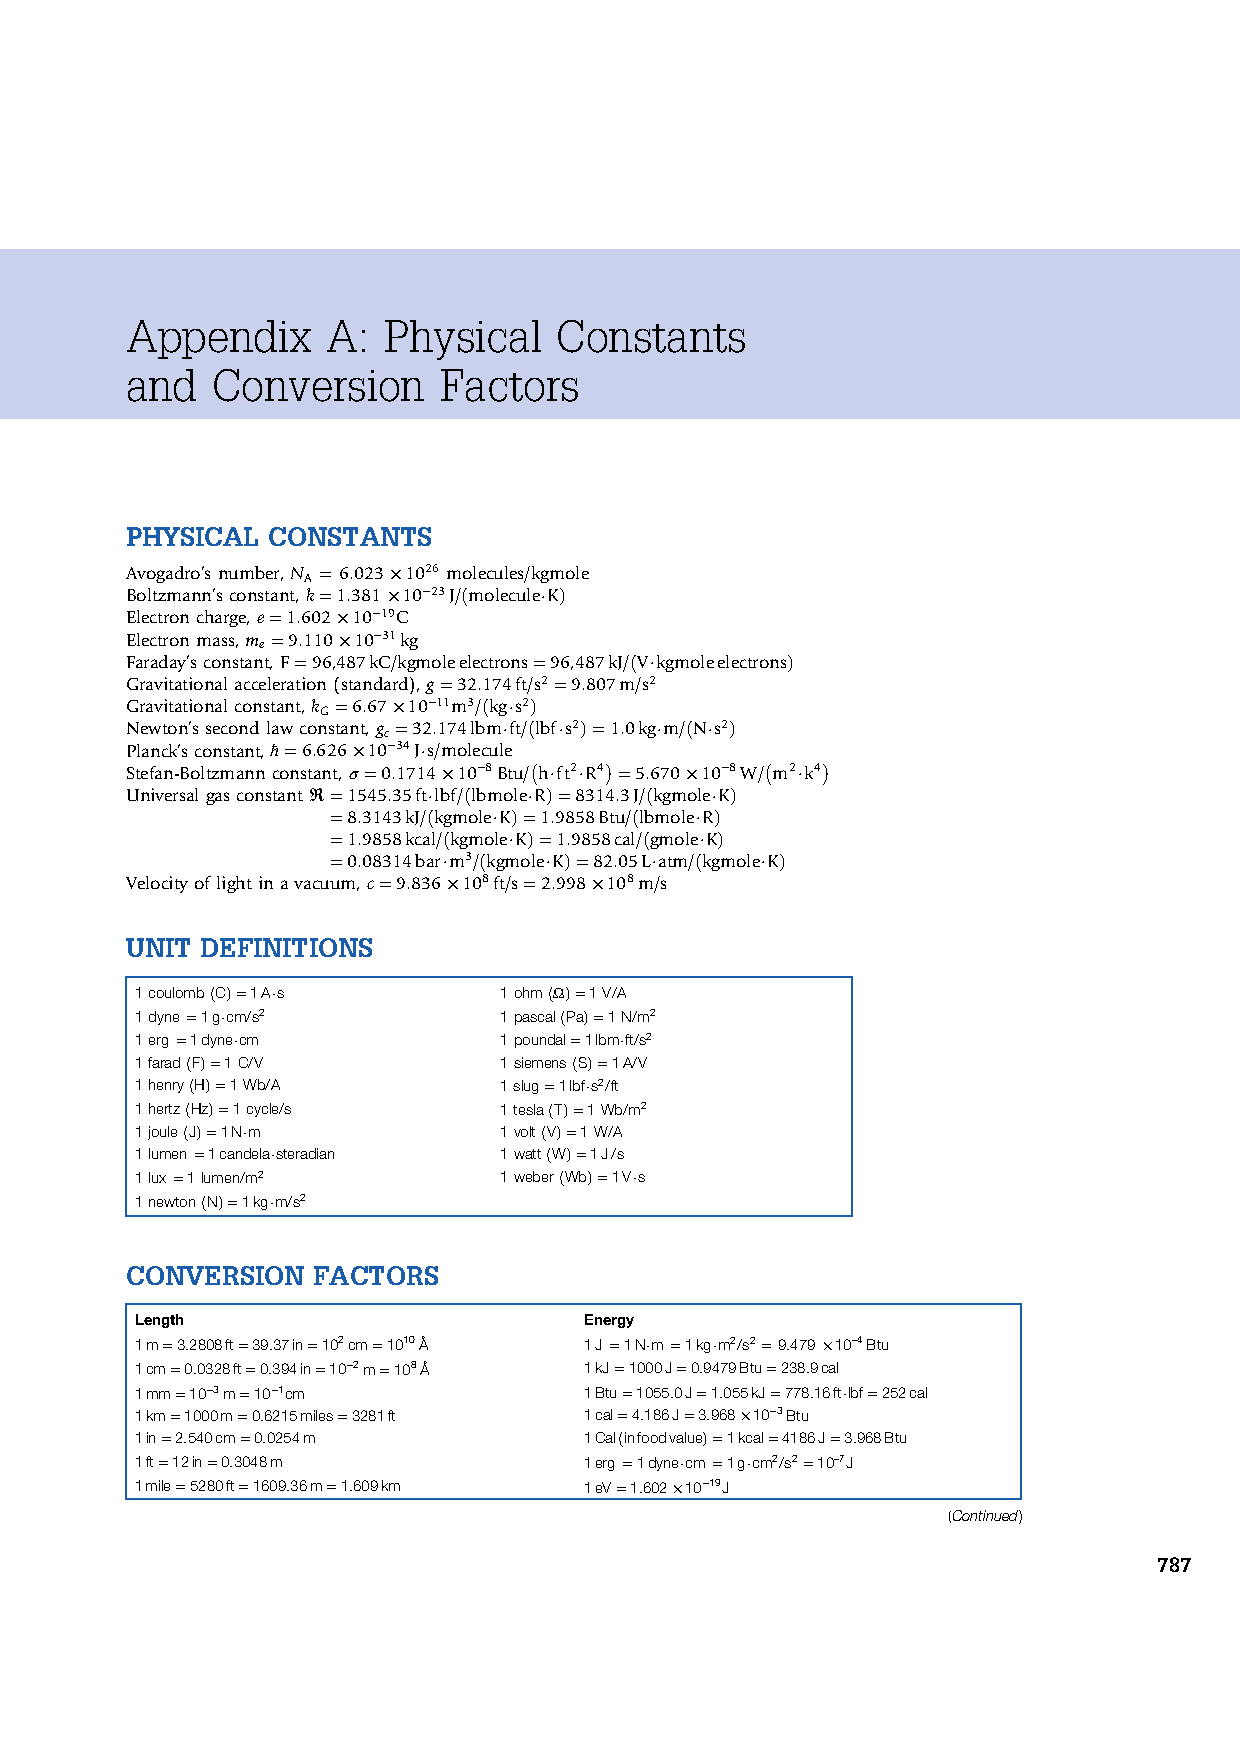
\includepdf[pages=-,fitpaper]{./Pics/ChemEng_UnitConv}
  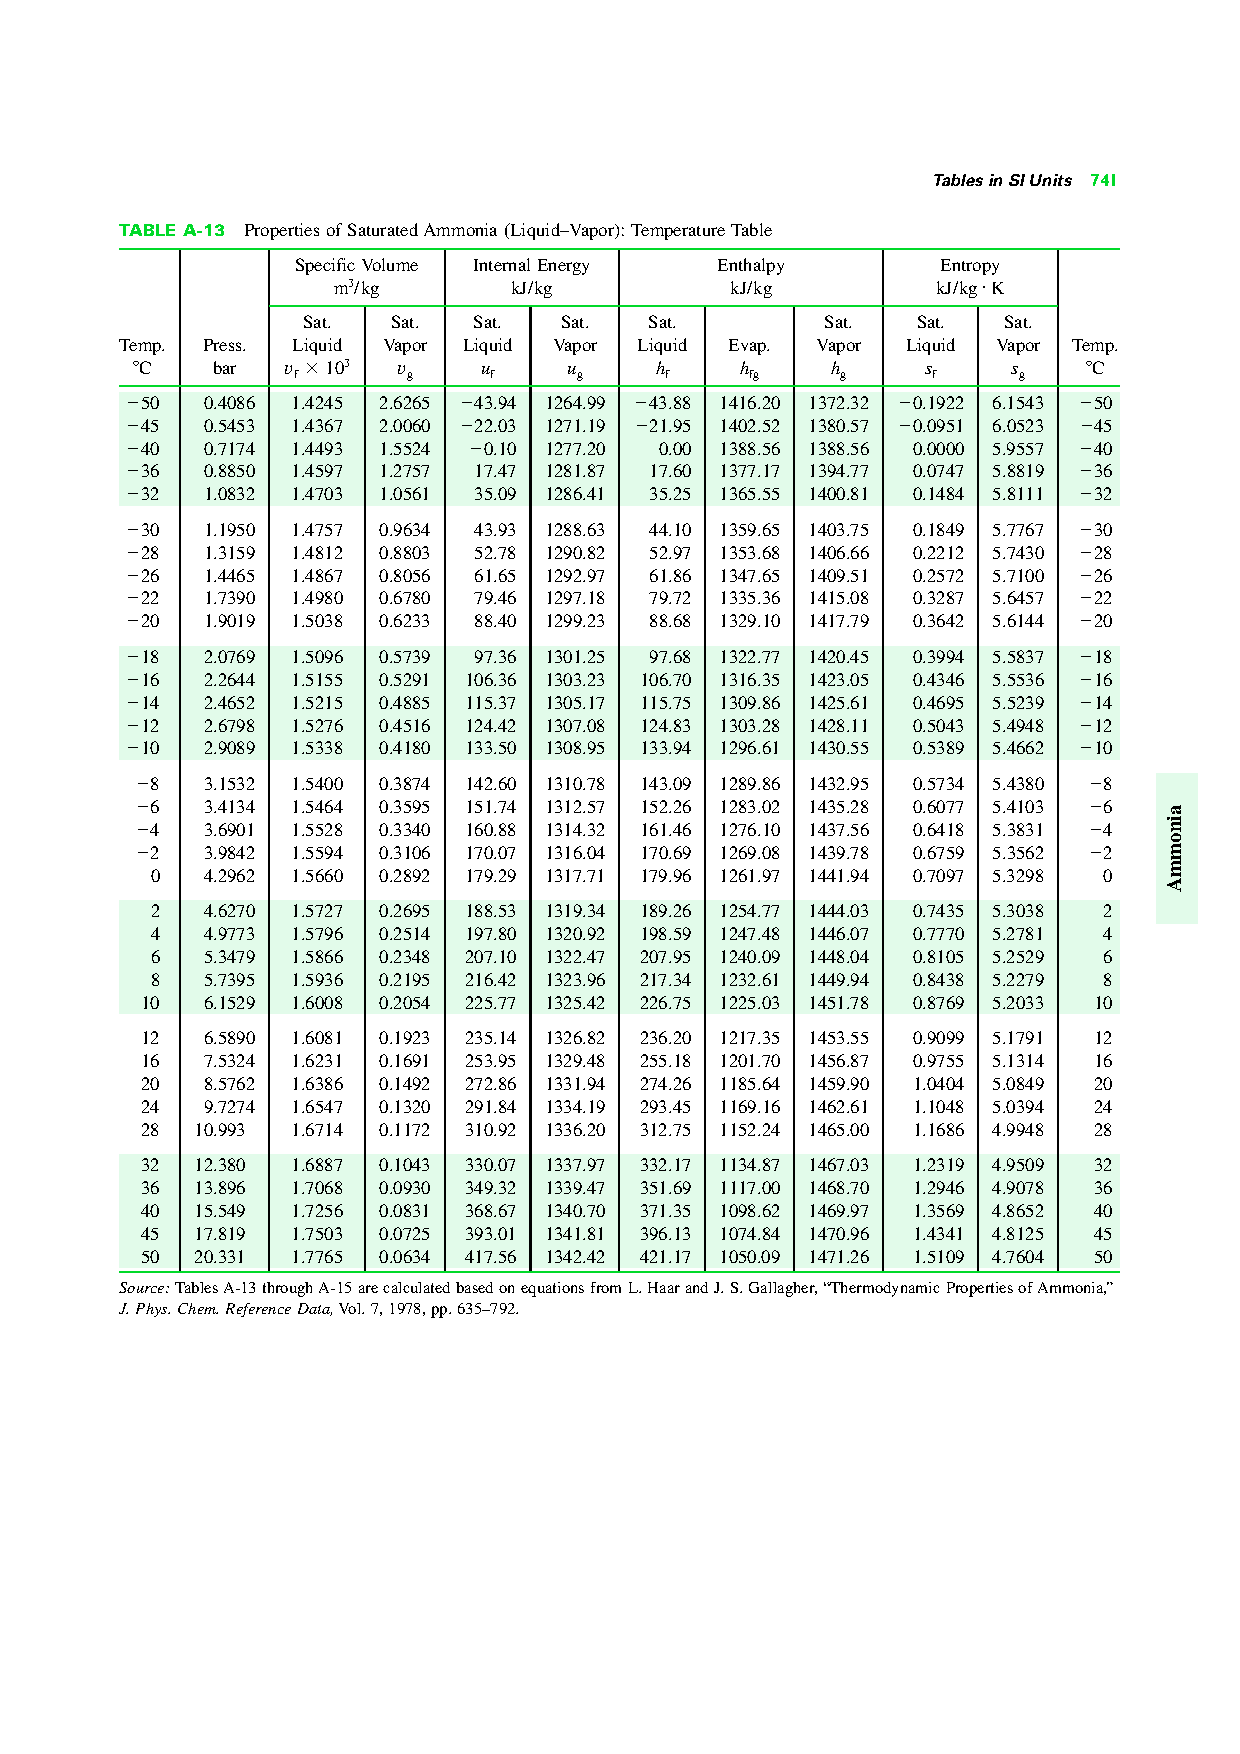
\includepdf[pages=-,fitpaper]{./Pics/ChemEng_NH3Tables}
}


\end{document}
